%
% This is the LaTeX template file for lecture notes for EE 382C/EE 361C.
%
% To familiarize yourself with this template, the body contains
% some examples of its use.  Look them over.  Then you can
% run LaTeX on this file.  After you have LaTeXed this file then
% you can look over the result either by printing it out with
% dvips or using xdvi.
%
% This template is based on the template for Prof. Sinclair's CS 270.

\documentclass[twoside]{article}
\usepackage{graphics}
\setlength{\oddsidemargin}{0.25 in}
\setlength{\evensidemargin}{-0.25 in}
\setlength{\topmargin}{-0.6 in}
\setlength{\textwidth}{6.5 in}
\setlength{\textheight}{8.5 in}
\setlength{\headsep}{0.75 in}
\setlength{\parindent}{0 in}
\setlength{\parskip}{0.1 in}

%
% The following commands set up the lecnum (lecture number)
% counter and make various numbering schemes work relative
% to the lecture number.
%
\newcounter{lecnum}
\renewcommand{\thepage}{\thelecnum-\arabic{page}}
\renewcommand{\thesection}{\thelecnum.\arabic{section}}
\renewcommand{\theequation}{\thelecnum.\arabic{equation}}
\renewcommand{\thefigure}{\thelecnum.\arabic{figure}}
\renewcommand{\thetable}{\thelecnum.\arabic{table}}

%
% The following macro is used to generate the header.
%
\newcommand{\lecture}[4]{
   \pagestyle{myheadings}
   \thispagestyle{plain}
   \newpage
   \setcounter{lecnum}{#1}
   \setcounter{page}{1}
   \noindent
   \begin{center}
   \framebox{
      \vbox{\vspace{2mm}
    \hbox to 6.28in { {\bf EE 382V: Parallel Algorithms
                        \hfill Fall 2017} }
       \vspace{4mm}
       \hbox to 6.28in { {\Large \hfill Lecture #1: #2  \hfill} }
       \vspace{2mm}
       \hbox to 6.28in { {\it Lecturer: #3 \hfill Scribe: #4} }
      \vspace{2mm}}
   }
   \end{center}
   \markboth{Lecture #1: #2}{Lecture #1: #2}
   %{\bf Disclaimer}: {\it These notes have not been subjected to the
   %usual scrutiny reserved for formal publications.  They may be distributed
   %outside this class only with the permission of the Instructor.}
   \vspace*{4mm}
}

%
% Convention for citations is authors' initials followed by the year.
% For example, to cite a paper by Leighton and Maggs you would type
% \cite{LM89}, and to cite a paper by Strassen you would type \cite{S69}.
% (To avoid bibliography problems, for now we redefine the \cite command.)
% Also commands that create a suitable format for the reference list.
\renewcommand{\cite}[1]{[#1]}
\def\beginrefs{\begin{list}%
        {[\arabic{equation}]}{\usecounter{equation}
         \setlength{\leftmargin}{2.0truecm}\setlength{\labelsep}{0.4truecm}%
         \setlength{\labelwidth}{1.6truecm}}}
\def\endrefs{\end{list}}
\def\bibentry#1{\item[\hbox{[#1]}]}

%Use this command for a figure; it puts a figure in wherever you want it.
%usage: \fig{NUMBER}{SPACE-IN-INCHES}{CAPTION}
\newcommand{\fig}[3]{
			\vspace{#2}
			\begin{center}
			Figure \thelecnum.#1:~#3
			\end{center}
	}
% Use these for theorems, lemmas, proofs, etc.
\newtheorem{theorem}{Theorem}[lecnum]
\newtheorem{lemma}[theorem]{Lemma}
\newtheorem{proposition}[theorem]{Proposition}
\newtheorem{claim}[theorem]{Claim}
\newtheorem{corollary}[theorem]{Corollary}
\newtheorem{definition}[theorem]{Definition}
\newenvironment{proof}{{\bf Proof:}}{\hfill\rule{2mm}{2mm}}

% **** IF YOU WANT TO DEFINE ADDITIONAL MACROS FOR YOURSELF, PUT THEM HERE:

\begin{document}

%FILL IN THE RIGHT INFO.
%\lecture{**LECTURE-NUMBER**}{**DATE**}{**LECTURER**}{**SCRIBE**}
\lecture{6}{August 19}{Vijay Garg}{Kelsey Sandlin}
%\footnotetext{These notes are partially based on those of Nigel Mansell.}

% **** YOUR NOTES GO HERE:
\section{Introduction}
This document presents the material from Chapter 8 that was covered in lecture 6. The topic is mutual exclusion
in distributed systems, and Lamport's Algorithm and Ricart and Agrawala's algorithm are given as possible solutions.
\section{Mutual Exclusion in Distribued Systems}
There often exisits some functionality that will only consistently produce correct output if limited to one
process at a time. We can use a chat program (assume it looks like a live document and there is no conflict resolution) as an example:
Two users should not be able to type at the same time or conflicts will occur. Typing should be considered the "Critical Section". \\
\textbf{Critical Section Properties}
\begin{enumerate}
    \item \textbf{Safety} -- two processes should not be in the critical section at the same time
    \item \textbf{Liveness/Progress} -- every request to enter the critical section should eventually be granted
    \item \textbf{Fairness} -- requests are granted in the order they are made. Fairness definitions may vary.
\end{enumerate}

It is trivial to implement safety without the liveness or fairness constraints -- don't let any process into the critical section.

\section{How do we solve the mutual exclusion problem?}
\subsection{Assumptions}
\begin{itemize}
    \item N total processes
    \item completely connected topology \& FIFO
    \item no faulures (solution does not need to be fault tolerant)
\end{itemize}
\subsection{Brainstorming}
We can't use a single shared lock because there is no shared memory.
We need a queue structure to hold the requests to the critical section.
Let's designate one server to manage the critical section and queue of requests.
\section{Centralized Solution}
The dedicated server maintains a queue of requests by adding each request received to the end of the queue.
We assume that when a process is done with the critical section, it always alerts the dedicated server and the dedicated
 server then allows the next process in the queue to enter. \\
This solution satisfies \textbf{safety} and \textbf{liveness}, but not necessarily \textbf{fairness}. This is because
processes are added to the queue in the order they are \textit{received}, which is not necessarily the order the
requests are sent. \par
We can make this solution fair by sending vector clocks along with the request. The dedicated server would insert
requests into the queue in order by their process time. \par
\textbf{But this solution really isn't distributed.}

\section{Lamport's Algorithm}
In order to extend the centralized solution to be distributed, all processes need to maintain a queue of requests. \\
\[\textbf{queue structure:} ((p1 LCV, 1), (p9 LCV, 9), (p4 LCV,4)) \]
Where LCV = Logical Clock Value (Lamport's Clock Value) and the second value in each tuple is pid \\
A process is considered to be first in the queue if it's LCV is less than all other processes LCVs in the queue. It is
possible that two or more processes send their request at the same LCV. In this case, you use resolve by selecting the
lower pid value. \\
\\
*How can we guarantee that all processes have identical queues? \\

\textbf{Lamport's Algorithm Psuedocode} \\
P\textsubscript{i} can enter it's critical section if:
\begin{enumerate}
    \item P\textsubscript{i}'s request is the smallest in the queue
    \item P\textsubscript{i} has received acks from all other processes
\end{enumerate}
\underline{request:}
\begin{enumerate}
    \item Enter your request (LCV,pid) into your local queue
    \item Send request message to all other processes including LCV and pid
\end{enumerate}
\underline{receive request:}
\begin{enumerate}
    \item Add P\textsubscript{i}'s request to local queue
    \item Send ack to P\textsubscript{i}
\end{enumerate}
\underline{release:}
\begin{enumerate}
    \item Remove request from the queue
    \item Send "release" message to all other processes (include pid)
\end{enumerate}
\underline{receive release:}
\begin{enumerate}
    \item Remove P\textsubscript{i}'s request from the queue
\end{enumerate}

\textbf{Does Lamport's algorithm satisfy the mutual exclusion properties?}
\begin{itemize}
    \item \textbf{Safety}
\end{itemize}
Let's assume P\textsubscript{i} and P\textsubscript{j} are in the CS at the same time and LVC\textsubscript{j} is less than
LVC\textsubscript{i}. In order for P\textsubscript{j} to have entered the CS, P\textsubscript{i} must have seen an ack
from P\textsubscript{j}. P\textsubscript{j} could have sent the ack to  P\textsubscript{i} either before or after sending
it's request message. \\
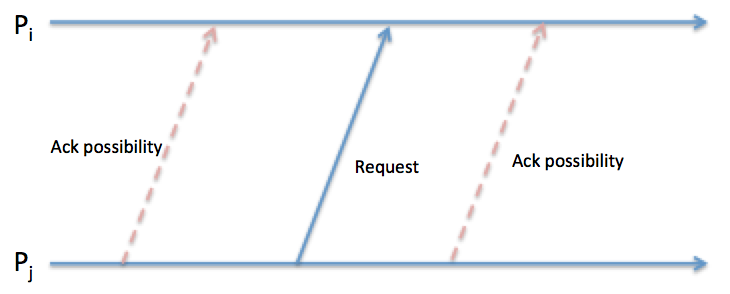
\includegraphics{lamportSafety.png} \\
P\textsubscript{j} could not have sent the ack before the request because that would mean mean
P\textsubscript{i}'s request must have already happened (which would have forced P\textsubscript{j}'s LVC to update),
but that contradicts our assumption that LVC\textsubscript{j} is less than LVC\textsubscript{i}. \\
If the ack to P\textsubscript{i} is sent after the request, then (by FIFO property) P\textsubscript{i} must
have seen P\textsubscript{j}'s request prior to P\textsubscript{j}'s ack and would have P\textsubscript{j}'s request
in the queue before it's own request and therefore not entered the CS
\begin{itemize}
    \item \textbf{Liveness and Fairness}
\end{itemize}
In Lamport's Algorithm, all requests are granted in the order of logical clock value. Assuming no message failures,
liveness and fairness are guaranteed. \\

\textbf{Analysis}
Requires 3(N-1) messages for N processes
\begin{itemize}
    \item N-1 messages to send a request
    \item N-1 messages to send ack
    \item N-1 messages to send release
\end{itemize}

How can we reduce the number of messages sent? In the next algorithm we will combine "ack" and "release" messages into
one message: "okay".


\section{Ricart and Agrawala's Algorithm}
The main idea is that there is no need for P\textsubscript{i} to to send an ack when receiving a request from
P\textsubscript{j} if P\textsubscript{i} knows his reqest is before P\textsubscript{j}'s request.
Instead of each process keeping track of all the current requests, they now keep a \textit{pending} queue that contains
the requests that have been received \textbf{but not acknowledged}. \\

\textbf{R\&A's Algorithm Psuedocode} \\
P\textsubscript{i} can enter it's critical section if:
\begin{enumerate}
    \item P\textsubscript{i} has received "okay" messages from all other processes
\end{enumerate}
\underline{request:}
\begin{enumerate}
    \item Send request message to all other processes including LCV and pid
\end{enumerate}
\underline{receive request from P\textsubscript{j}:}
\begin{enumerate}
    \item If P\textsubscript{i} is not requesting the CS or if P\textsubscript{j}'s request's timestamp is less than
    P\textsubscript{i}'s request: Send "okay" to P\textsubscript{j}
    \item Else: Insert P\textsubscript{j} into the pending queue
\end{enumerate}
\underline{release:}
\begin{enumerate}
    \item Send "okay" message to all processes in the pending queue
\end{enumerate}

\textbf{Does R\&A's algorithm satisfy the mutual exclusion properties?}
\begin{itemize}
    \item \textbf{Safety}
\end{itemize}
Let's assume P\textsubscript{i} and P\textsubscript{j} are in the CS at the same time and LVC\textsubscript{j} is less than
LVC\textsubscript{i}. In order for P\textsubscript{j} to have entered the CS, it must have seen "okay" from
from P\textsubscript{i}. We know the request from P\textsubscript{i} must have been received by P\textsubscript{j}
after P\textsubscript{j} had made it's request, otherwise the LCV of P\textsubscript{j} would be greater than
the LVC of P\textsubscript{i}. At this point, if P\textsubscript{j} were in the CS, it would hold it's "okay" until
after exiting the CS (by the algorithm) and P\textsubscript{i} would not be allowed in. If P\textsubscript{j} is not
in the CS, it would still realize P\textsubscript{i}'s higher LCV and hold it's "okay".
\begin{itemize}
    \item \textbf{Liveness and Fairness}
\end{itemize}
All requests are granted in the order of logical clock value. Assuming no message failures,
liveness and fairness are guaranteed. \\

\textbf{Analysis}
Requires 2(N-1) messages for N processes
\begin{itemize}
    \item N-1 messages to send a request
    \item N-1 messages to send "okay"
\end{itemize}

\end{document}
